%% bt: Bachelor Thesis
%% mt: Master Thesis
\documentclass[bt]{dbvdoc}

% Alternative Loesunge:
% - use utf8 on your home computer
% - use an editor capable of converting character-sets and editing utf8 files
%   on a latin1 system (some versions of vi do)
% - use \"{a}, \"{o}, \"{u}, \ss{} instead of non-ascii characters

\usepackage[utf8]{inputenc}
%%\usepackage[utf8,latin1]{inputenc}  %% Alternative Eingabe
\usepackage[ngerman, english]{babel}
\usepackage[babel,german=quotes]{csquotes}
\usepackage[backend=biber,maxnames=99,language=english,bibstyle=alphabetic,sortcites=true,labelalpha=true,style=alphabetic]{biblatex}
\usepackage{hyperref}
\usepackage{breakurl}
%\usepackage[hyphenbreaks]{breakurl}  %% Falls in \url auch bei Bindestrich getrennt werden soll. Weitere Optionen: RTFM
\usepackage{graphicx}
\usepackage{epsfig}
\usepackage{subfigure}
\usepackage{psfrag}
\usepackage{color}
\usepackage{amsmath}
\usepackage{tikz}
\usepackage{tikz-cd}
\usepackage{pgfplots}
\pgfplotsset{compat=1.14}
% workaround for matplotlib pgf plots
\def\mathdefault#1{#1}
\usepackage{svg}
% Hurenkinder/Schusterjungen ausschliessen
\usepackage{nowidow}
\setnowidow[2]
\setnoclub[2]
\usepackage{listings}
\lstdefinestyle{pseudocode}{frame=lr}
\lstset{style=pseudocode,captionpos=b,frame=tb}
\renewcommand{\lstlistlistingname}{List of Listings}

% \setcounter{lotdepth}{2}

% ++ es werden keine underfull hboxes als Fehler ausgegeben,
%    da das ja nur heißt, dass die Seite noch nicht ganz voll ist
\hbadness=10000
\clubpenalty = 10000 % schliesst Schusterjungen aus
\widowpenalty = 10000 % schliesst Hurenkinder aus

\pagenumbering{roman}

%\bibliographystyle{amsalpha}
\renewcommand*{\labelalphaothers}{\textsuperscript{}} %% plus-zeichen abschalten
\bibliography{doc}
\addbibresource{doc.bib}

%%%%%%%%%%%%%%
%%% MACROS %%%
%%%%%%%%%%%%%%
%% if macros shall be used, put them into a separate file 'macros.tex'
%%\input{macros}

%%%%%%%%%%%%%%%%%%%%
%%% Worttrennung %%%
%%%%%%%%%%%%%%%%%%%%
%% if hyphenation patterns are needed, put them into a separate file 'hyph.tex'
%%\input{hyph}


%%%%%%%%%%%%%%
%\setcounter{tocdepth}{5}
%\setcounter{secnumdepth}{5}

\sloppy		%% avoid writing over linebreak


\begin{document}
\clearpage
  \begin{deckblatt}
    \Titel{Simulating Room Acoustics Using Ray Tracing}
    \Name{Reichel}
    \Vorname{Christina}
    \Wohnort{Würzburg}
    \BetreuerA{Erstpr\"{u}fer: Prof.~Dr.-Ing.~Frank Deinzer}
    \BetreuerB{Zweitpr\"{u}fer: Prof.~Dr.-Ing.~Arndt Balzer}
    \Ende{02. 04. 2024}
    \Fach{Informatik}
    \Schwerpunkt{Medieninformatik}
    \Angefertigt{Angefertigt an der Fakultät für Informatik und Wirtschaftsinformatik der Technischen Hochschule Würzburg-Schweinfurt}
  \end{deckblatt}
\clearpage
\mbox{}
\vfill
\begin{center}
\ifpdf
	
\includegraphics[width=6cm]{qrcode-thesis.png}
\else
	
\includegraphics[width=6cm]{qrcode-thesis.eps}
\fi
\end{center}
\clearpage

\noindent Hiermit versichere ich, dass ich die vorgelegte Bachelorarbeit/Masterarbeit selbstständig verfasst und noch nicht
anderweitig zu Prüfungszwecken vorgelegt habe. Alle benutzten Quellen und Hilfsmittel sind
angegeben, wörtliche und sinngemäße Zitate wurden als solche gekennzeichnet.\\[5mm]
Würzburg, den\\[20mm]
(Unterschrift)

\vfill

\noindent Hiermit willige ich ein, dass zum Zwecke der Überprüfung auf Plagiate meine vorgelegte Arbeit in
digitaler Form an PlagScan übermittelt und diese vorübergehend (max. 5 Jahre)
in der von PlagScan geführten Datenbank gespeichert wird, sowie persönliche Daten, die Teil dieser
Arbeit sind, dort hinterlegt werden.

Die Einwilligung ist freiwillig. Ohne diese Einwilligung kann unter Entfernung aller persönlichen
Angaben und Wahrung der urheberrechtlichen Vorgaben die Plagiatsüberprüfung nicht verhindert
werden. Die Einwilligung zur Speicherung und Verwendung der persönlichen Daten kann jederzeit
durch Erklärung gegenüber der Fakultät widerrufen werden.\\[5mm]
Würzburg, den\\[20mm]
(ggf. Unterschrift)

\clearpage

\begin{center}
\bf Übersicht
\end{center}
Existierende Forschung zu Akustiksimulation befasst sich fast ausschließlich mit der Simulation statischer Szenen.
Dynamische oder sich bewegende Szenen werden höchstens simuliert,
indem die Szene kurzzeitig gestoppt wird und der Raumhall in dieser gestoppten Szene berechnet wird.
In dieser Arbeit wird eine Methode entwickelt,
mit der Szenen mit beweglichen Objekten korrekt modelliert werden können,
und einige Optimierungen für diese geprüft.
Somit wird ein Grundstein für korrekte Simulation nicht-statischer Szenen gelegt.

\vfill
\begin{center}
\bf Abstract
\end{center}
Existing research into acoustics simulation has almost exclusively concerned itself with static scenes.
Dynamic or moving scenes are at best simulated by temporarily stopping the scene's movement
and calculating that static snapshot scene's reverberation.
This thesis proposes a method to correctly model scenes with moving objects,
then also looks into optimising this method's performance.
This lays part of the foundation for correct simulation of non-static scenes.

\vfill
\cleardoublepage

\tableofcontents

\cleardoublepage \pagenumbering{arabic}

%%%%%%%%%%%%%%%%%%%%%%%
%%% Include chapter %%%
%%%%%%%%%%%%%%%%%%%%%%%
\chapter{Introduction}

\section{Motivation}

While there has been plenty of research into simulating sound propagation using both geometric and numerical methods,
nearly all of it only concerns itself with static scenes,
where neither objects within the scene nor the sound emitter nor receiver move with time.
\newline
Simulation of dynamic or moving scenes is mostly unexplored.
This is mostly because it is only really relevant for scenarios
where objects or receivers can move at speeds within one or two orders of magnitude from the ray's travelling speed;
If this condition is not fulfilled,
the error introduced from the snapshot method described below becomes minimal enough to be disregarded.
\newline
For light, the travelling wave relevant to computer graphics, this condition does not apply as
light famously travels at approximately \(3 \cdot 10^{8} m/s\).
As a reference, the fastest velocity achieved by humans is approximately \(1.1 \cdot 10^4 m/s\) during the launch of Apollo 10.
Seeing as even this extreme case is four orders of magnitude smaller than the speed of light,
errors introduced to computer graphics by the snapshot method are especially small.
\newline
Only a comparatively small part of the research into ray tracing comes from outside of computer graphics to begin with,
and even in other fields, such as acoustics simulation,
the error introduced by the snapshot method is only relevant in edge cases.
All of this makes simulation of moving scenes a rather niche problem.
\newline
Despite this, some research into simulating moving or dynamic scenes' acoustics has been done:
\newline
Raghuvanshi et al.~\cite{RS10} explore a numerical approach to handle dynamically moving emitters and receivers,
but do not look into moving objects within the scene.
\newline
Chandak et al.~\cite{Cha08} attempt to simulate dynamic scenes in real-time,
with support for dynamically moving scenes but sacrificing accuracy.
This is less exploring how to handle moving scenes
and more exploring methods to run acoustics simulation fast enough
to re-calculate acoustics at a similar rate to that at which objects move by significant amounts.
\newline
% TODO: cite EAR
Similarly, EAR, an acoustics simulation tool based on the 3d modelling software blender,
allows for moving scenes through blender's keyframe system,
but is inaccurate for the same reason as Chandak's real-time approach:
\newline
Both EAR and Chandak et al.\ approach the simulation of moving scenes by taking a static version of the scene
at the time rays are emitted to create an impulse response,
then bouncing rays through this static snapshot.
This approach will be called the snapshot method in this thesis.
\newline
The snapshot method comes with a few advantages:
As the snapshot is just a static scene,
the same well-explored and -optimised bouncing logic used for static scenes can be copied without changes.
Also, crucially, knowledge of how the scene will move over the time the ray spends bouncing around it is not required.
All data necessary to simulate the bouncing is available at the time the ray is emitted,
without a need for information on how the scene will continue to move.
This is especially helpful for real-time simulation of dynamic scenes, as data about how the scene will continue to move is not
fully known at runtime.
\newline
\begin{figure}\label{SnapshotExplain}
    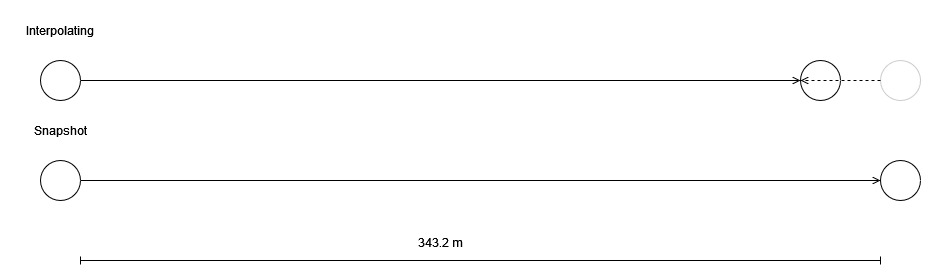
\includegraphics[width=\linewidth]{images/snapshot_explain.jpg}
    \caption{Difference between ray travelling distance using the newly developed interpolating method (top) as opposed to the snapshot method (bottom). In the interpolated version, the ray only travels part of the distance as the receiver travels the remainder.}
\end{figure}
The major downside of this snapshot approach is that it tends to introduce errors when objects or receivers move at high speeds.
As a simple example case, take the scene described in~\ref{SnapshotExplain}:
A receiver starts 343 meters away from an emitter and moves towards it at 1/9th the speed of sound, roughly 38 meters per second
(137.2 kilometers per hour, a speed most modern cars can reach without problems).
\newline
Using the snapshot approach, a ray traveling directly from emitter to receiver would arrive after travelling the full 343 meters,
taking 1 second for it to arrive at the receiver.
In actuality, in the time the ray takes to travel the first 90\% of that distance,
the receiver has already travelled the remaining 10\%, making for a response time of 0.9 seconds rather than 1 second.
\newline
While Bilibashi et al.~\cite{BVD20} have attempted to solve this issue,
they only aimed to simulate waves bouncing between a few set points, namely cars,
rather than simulating full room acoustics.
Their vector-based approach cannot be used for a full scene simulation.
\newline
To accurately simulate both edge cases occurring in the real world (such as the example above)
and hypothetical situations such as the test cases described below,
a new method needs to be developed.

\section{Scope}

This thesis proposes a method to simulate rays bouncing through arbitrary scenes with moving receivers and/or objects,
assuming all movement within the scene is known at time of calculation.
An improved way of checking for intersections between rays and objects is developed, accommodating for this new requirement.
Optimisations are evaluated and a time-based chunking method is developed to avoid needless intersection checks.
Additionally, a method is developed to to losslessly and efficiently store the multiple impulse responses created by re-calculating
the impulse responses for different points in time.
The goal of this research is to simulate effects such as the situation described in~\ref{SnapshotExplain} without errors introduced by the snapshot method
as well as recreate the acoustics of a hypothetical, rapidly rotating room.
Three test cases are developed for this and compared to an implementation of the snapshot method:
An empty scene with the sound receiver approaching the sound emitter at 1/9th the speed of sound,
a square room rapidly rotating
and a large, L-shaped room also rapidly rotating around one of its ends, with the receiver and emitter both sitting in said end.
\newline
Not within the scope of this thesis is a fully accurate simulation
including effects such as the differing bouncing behaviour sound waves show at different frequencies.
Only a proof of concept that shows that the idea of this new simulation method works is developed.
\newline
Side effects of moving scenes, such as sounds emitted by moving objects, are also discarded as they are irrelevant to
the changed intersection logic.
A note-worthy side effect that gets ignored is mass inertia:
The example case where this would become relevant is the inside of a linearly moving enclosed room, such as a driving car.
Due to mass inertia, sound waves travelling inside this moving rome behave the same as if the car stood still.
Since this effect is only relevant in a niche scenario and it can be simulated using a method that ignores movement entirely,
it can be ignored for this research.
\newline
Real-time applications cannot use this proposed method as it requires knowledge of objects' future movements ahead of time.
Further research is required to develop an alternative method for real-time or dynamic simulations.
A real-time approach could work by not calculating the rays' entire movements at emission time,
but instead keeping track of all moving rays and incrementally continuing their journey through the now updated scene
at recurring intervals.

\cleardoublepage
\chapter{Fundamentals}\label{ch:Fundamentals}

In order to be able to make use of the findings in this thesis,
A basic understanding of ray tracing both in general as well as in the context of acoustics simulation is required.
This chapter will provide a summary of the base idea of ray tracing
before then introducing specific concepts relevant to acoustics.

\section{Ray Tracing}\label{sec:FundamentalRT}

Both sound and light are generally known to be waves bouncing from wall to wall.
They start out from some emitter such as a loudspeaker and can eventually,
after bouncing off walls for any number of times, arrive at a receiver such as a microphone or an ear.
Ray tracing attempts to model this process of waves bouncing by splitting a wave into many individual rays,
each launched from the wave's emitter in a direction the wave would travel in too.
Most audio ray tracers assume emitters emit sound uniformly in all directions,
thus allowing them to simply launch each ray in a randomised direction.
\newline
Each ray's journey through the scene is then individually simulated
by calculating which object it will next intersect with,
then calculating the intersection point and the direction the ray will bounce off the object in.
Then, a new ray in the resulting direction is launched from this intersection point and the process is repeated
until some ending condition applies, at which point the ray is terminated.
If the ray intersects with a receiver object, the according information gets stored.
For acoustics, this is usually the intersection time and the energy the ray still had at intersection time.
Depending on the domain, the ray is then terminated or continues bouncing by passing through the receiver.
For acoustics, the latter behaviour is usually used.
\newline
Intersection checks are usually done by modelling objects using an equation that describes whether a point is on the object surface or not,
then injecting the ray's function into that equation and resolving.
With static objects, this check is trivial:
The only parameter to resolve for is the intersection time \(t\), and said parameter only occurs in the ray function,
usually making for a first-degree polynomial function.
\newline
As an example, a surface \(S\) can be modelled using a point \(P_1\) on it as well as its normal \(n\).
Then, to tell if any point \(p\) is on \(S\), the vector from \(P_1\) to \(p\) can be compared to \(n\).
If they're orthogonal to each other (thus their dot product is 0), \(p\) is on \(S\):

\begin{equation}\label{StaticSurface}
    (p - P_1) \cdot n = 0
\end{equation}

For a polygon defined by its corner points \(P_{1}\) to \(P_{m}\), the same equation can be used,
with the difference that \(n\) needs to be determined from a set of at least three of the points.
The cross product of two vectors is always orthogonal to both vectors, so using three points \(P_{1}\) through \(P_{3}\),
\(n\) can be determined as

\begin{equation}\label{PolygonNormal}
    n = (P_{2} - P_{1}) \times (P_{3} - P_{1})
\end{equation}

Additionally, a polygon needs to further check whether \(p\) is actually inside the bounds defined by its corners.
For triangles, this can be done using barycentric coordinates.
\newline
\begin{figure}[t!]
    \begin{center}
    \includesvg{images/barycentric.svg}
    \end{center}
    \caption{The barycentric coordinates of a point inside a triangle. Each coordinate is determined by the area of its subtriangle in relation to the whole triangle.}\label{fig:BarycentricExplain}
\end{figure}
Barycentric coordinates describe a point on a triangle (or another simplex) by separating a triangle into three parts,
each with the given point and two corners of the triangle as its vertices.
Each coordinate then describes the relative size of that subtriangle with respect to the full triangle,
as shown in \autoref{fig:BarycentricExplain}.
\newline
Thus, each point inside the triangle can be described by coordinates \((\alpha, \beta, \gamma)\),
with \(0 \le \alpha \le 1\), \(0 \le \beta \le 1\), \(0 \le \gamma \le 1\) and \(\alpha + \beta + \gamma = 1\).
If these conditions do not apply to \(p\), it is outside the triangle.
\newline
The naive way to calculate barycentric coordinates would be to calculate the areas of \(P_1P_2p\), \(P_1P_3p\), \(P_2P_3p\) and
divide them by the area of \(P_1P_2P_3\)~\cite{SM09}:
\begin{verbatim}
    normal = cross((p3 - p1), (p2 - p1));
    p1p2p = dot(normal, cross((p1 - p), (p2 - p)));
    p1p3p = dot(normal, cross((p3 - p), (p1 - p)));
    p2p3p = dot(normal, cross((p2 - p), (p3 - p)));
    p1p2p3 = p1p2p + p1p3p + p2p3p;
    alpha = p2p3p / p1p2p3;
    beta = p1p3p / p1p2p3;
    gamma = p1p2p / p1p2p3;
\end{verbatim}
This can be simplified by only computing two of the barycentric coordinates
and calculating the last one from the first two instead; if \(\alpha\) and \(\beta\) have already been computed,
\(\gamma = 1 - \alpha - \beta\). This saves a division operation.
For further optimisation, the Lagrange identity \((a \times b) \cdot (c \times d) = (a \cdot c)(b \cdot d) - (a \cdot d)(b \cdot c)\)
can be used to replace the cross products with dot products, as shown by Ericson~\cite{Er04}.
\newline
In order to calculate the intersection point \(p\), the equation describing a ray then needs to be injected into the surface equation.
A ray \(R\)'s position at time \(t\), with \(R\) starting at the point \(P\) at time \(t_0\)
and travelling in the direction \(v\) can be defined as follows:

\begin{equation}\label{RayEq}
    R(t) = P + (t - t_0) \cdot v
\end{equation}

This equation can then be injected into the equation describing the primitive and resolved.
As an example, using~\eqref{StaticSurface}, this calculation goes as follows:

\begin{equation*}
    (P + (t - t_0) \cdot v - P_1) \cdot n = 0
\end{equation*}
\begin{equation}\label{StaticSurfaceIntersect}
    t = \frac{(P_1 + t_0 \cdot v - P) \cdot n}{v \cdot n}
\end{equation}

If \(t\) exists and is greater than \(t_0\),
the point \(p = R(t)\) describes the intersection point and can be used for further checks
as well as bouncing.
\newline
The bouncing direction can be determined in a number of ways,
depending on the surface and how it reflects waves.
The easiest to understand behaviour is specular reflection,
where angle of incidence equals angle of departure -
i.e. a ray bounces off of a surface in the same angle it approached it at,
such as when light bounces off a perfect mirror.
The specularly reflected direction \(r\) can be calculated from the inbound direction \(i\) and the surface normal \(n\) as
\begin{equation}\label{eq:SpecularReflection}
    r = i - (2 \cdot i \cdot n) \cdot n
\end{equation}
Different reflection modes will be discussed in \autoref{sec:FundamentalGA} as they are usually domain dependent
and not important for a general understanding of ray tracing.
\newline
Alongside the launch position and direction,
rays usually store the energy or colour information they represent in some form.
This information tends to get altered with each bounce -
For acoustics simulation, the ray's energy simply gets decremented depending on the bouncing material.
This too will be elaborated on in \autoref{sec:FundamentalGA}.
\newline
This stored energy can be used as an ending condition:
Once the ray's energy goes below a certain threshold,
the ray is terminated as any energy it carries becomes insignificant.
Other domains, where the ray's stored data cannot fully be used to determine its relevance,
use other ending conditions.
One simple condition often seen in computer graphics is bounce count:
Each ray also counts the amount of times it already bounced.
Once a specified threshold of bounces is reached, the ray is discarded.

\section{Acoustics Simulation}\label{sec:FundamentalAcoustics}

The goal of acoustics simulation is to get a picture of when sound waves arrive at a receiver and with what amount of energy.
A simulation creates either an impulse or energetic response,
which can in turn be used to determine acoustic properties of the room
or applied to a sound recording in order to simulate it being recorded in this room.
The latter process is called `auralization'.
\newline
One common measure for room properties is the reverberation time \(T_{60}\),
defined as the point after which the impulse/energetic response is consistently at least 60 decibels quieter than the initial signal.
This can be used as a metric to determine how long a sound will take to ring out in a room.
\newline
Another useful measure is the sound clarity \(C_{50}\)~\cite{AB18}~\cite{PMG22},
comparing the reverberation's first 50 milliseconds' worth of sound energy to the remainder of the reverberation.
\(C_{50}\) as a metric is based on the idea that for speech,
any reflections of the sound arriving more than 50 milliseconds later than the first response are harming intelligibility,
whereas signal arriving within that 50 millisecond window is helpful in making speech more understandable.
Thus, a higher \(C_{50}\) means that speech is easier to understand under the room's acoustic conditions.
\newline
For a known energetic response \(e_m, 0 \le m < o\), where each \(m\) represents one sample of the response and there are a total of \(o\) samples,
and a sample rate \(f\), \(C_{50}\) can be calculated as

\begin{equation}\label{eq:C50}
    C_{50} = 10 \cdot \log_{10} \left( \frac{\displaystyle\sum_{m=0}^{50 \cdot f - 1}e_m}{\displaystyle\sum_{m=50 \cdot f}^{o}e_m} \right) dB
\end{equation}

The impulse/energetic response of a room can usually be divided into three parts:
`direct sound' is the part of the sound wave that can immediately travel from emitter to receiver without bouncing off of a wall,
the `early reflections' are early, not yet diffuse echoes
and the remaining diffuse hall ringing out is called `late reverberation'.
\newline
The difference between an impulse and an energetic (or energy-time) response is the data being modelled.
An energy-based model produces an energetic response \(p^2(t)\).
This energy-time response is sufficient to make statements about a room's acoustics,
but cannot be used for proper auralization as phase information is lost.
The solution to this problem is provided by pressure-based models,
where instead of the energy \(p^2\),
the sound pressure \(p\) is computed as a complex number that also holds phase information.
\newline
As the energy response is the squared impulse response,
converting from the latter to the former is trivial.
The inverse conversion becomes more complicated as the phase information needs to be reconstructed,
usually from the ray's travelling distance.
\newline
For simplicity's sake, this thesis will only focus on energy-based models.
The concepts introduced can be equally applied to pressure-based models.

\section{Geometric Acoustics Simulation}\label{sec:FundamentalGA}

The changes to ray tracing specific to acoustics simulation mostly affect rays' bouncing behaviour.
Firstly, when a ray bounces off of a surface,
that surface will absorb part of the ray's energy.
How much of the incoming energy is reflected depends on the surface's impedance
as well as the angle of incidence \(\theta\).
\newline
For energy-based geometric acoustics, this is usually modelled through an absorption coefficient \(\alpha(\theta)\),
which in turn can be calculated from a wall's plane-wave reflection coefficient \(R(\theta)\) often determined through measurement.
Some systems simplify this to a single random incidence absorption coefficient \(\alpha_{rand}\)
computed as the average of all possible incidence angles.
\newline
Another important factor of acoustics that needs to be modelled is the effect of uneven surfaces.
Specifically, imperfections in a surface that are within the same order of magnitude as the wavelength greatly affect that surface's acoustic behaviour
as not waves are then not fully reflected in a specular manner.
These non-specular reflections are usually modelled in a simplified manner such as scattering coefficients.
\newline
The scattering coefficient, commonly noted as a number between 0 and 1, models the ratio of specularly to non-specularly reflected energy,
splitting the signal into a specular and a diffuse component.
A value of 0 means a perfectly even and specularly reflecting surface (like a perfect mirror for light),
whereas 1 implies a fully diffuse reflection.
\newline
The distribution of this diffuse reflection is not specified by the scattering coefficient,
so most systems simply assume a lambertian reflection model.
\newline
The naive way to implement this in a ray tracing system would be for a bounce to not just emit one new ray, but several,
with one keeping the specular component's energy and being reflected specularly,
while the diffuse component's energy is distributed among the remaining rays,
which in turn are randomly spread across the hemisphere defined by the surface normal.
This quickly becomes computationally expensive as the number of rays increases exponentially with each bounce.
\newline
In practice, to avoid the resulting performance problems,
some systems (such as EAR~\cite{Th17}) generate a random number between 0 and 1 for each collision.
If the scattering coefficient is greater than this random number,
the ray is sent off into a random direction in the hemisphere defined by the surface's normal,
otherwise it is reflected specularly as per \ref{eq:SpecularReflection}.
As a high amount of rays is sent out into the scene,
the result of this random distribution eventually matches the distribution defined by the scattering coefficient.
This is not as accurate as splitting up rays,
but usually accurate enough to be a justifiable optimisation.

\cleardoublepage
\chapter{Bouncing Rays Through Moving Scenes}\label{ch:Intersection}

To bounce a ray through a scene, checks need to be performed to know which objects it intersects with and thus bounces off of.
The general method for these intersection checks for static scenes has been established in \autoref{sec:FundamentalRT}.
\newline
Existing tools and research use this same method for intersection checks when simulating dynamic or moving scenes.
A snapshot copy of the scene at the time a ray is launched is made,
then intersection checks and bouncing logic use this static scene.
This approach to moving scenes will be called the `snapshot approach' or `snapshot method' in this thesis.
\newline
This snapshot approach comes with a few advantages:
The simple and well-optimised intersection logic from static scenes can be used without changes.
Also, crucially, knowledge of how the scene will move over the time the ray spends bouncing around it is not required.
All data necessary to simulate the bouncing is available at the time the ray is emitted,
without a need for information on how the scene will continue to move.
This is especially helpful for real-time simulation of dynamic scenes, as data about how the scene will continue to move is not
fully known at runtime.
\newline
\begin{figure}[t!]
    \includesvg[width=\linewidth]{images/snapshot.svg}
    \caption{Difference between ray travelling distance using the newly developed interpolating method (top) as opposed to the snapshot method (bottom). In the interpolated version, the ray only travels part of the distance as the receiver travels the remainder.}\label{im:SnapshotExplain}
\end{figure}
The major downside of this snapshot approach is that it tends to introduce errors when objects or receivers move at high speeds.
Take an example case of a sound receiver moving towards a sound emitter, as shown in~\autoref{im:SnapshotExplain}:
If the receiver starts at a distance \(d\) away from the emitter and sound travels at a speed \(c\),
the intersection time \(t\) becomes \(t = \frac{d}{c}\) as the receiver's movement is ignored.
In actuality, if the receiver moves towards the emitter at a speed \(v\), the calculation for the real \(t\) would be \(t = \frac{d}{c+v}\).
\newline
As an example case, say that \(d = 343.2m, c = 343.2 m/s, v = c/9 = 38.0\bar{2} m/s\)
(read: The receiver starts 1 second of travel at the speed of sound away from the emitter
and moves towards it at 1/9th the speed of sound).
\newline
Using the snapshot approach, a ray traveling directly from emitter to receiver would arrive after travelling the full 343.2 meters,
taking 1 second for it to arrive at the receiver.
In actuality, in the time the ray takes to travel the first 90\% of that distance,
the receiver will have already travelled the remaining 10\%,
making for a response time of \(t = \frac{343.2}{381.\bar{2}} = 0.9s\).
\newline
To avoid this issue, new intersection logic that takes objects' movements into account is needed.
This check becomes more complicated than its static counterpart as the equation describing the object still needs to be resolved for \(t\),
but now \(t\) is also part of the equation itself.
In this chapter, equations are established and solved to perform intersection checks with moving spheres and surfaces,
as those two should already be sufficient to simulate most scenes.
Equations for other primitives, such as quadric surfaces, should be derivable using a similar method.
\newline
The general scheme for this is as follows:
First, the object is modelled in a way where its position (or other parameters) is also a function of \(t\).
Then, like with a normal check, the function modelling the ray is injected into this equation,
then resolved.
This will, in the examples below, result in a polynomial function of a higher degree
(2nd and 3rd for spheres and surfaces, respectively), which can then be resolved.
\newline
Unlike with most ray tracing implementations, the magnitude of the ray's direction vector \(v\) becomes significant:
Since the movement of objects checked for intersections is also dependent on time,
objects and the ray must move at the same time scale.
\(v\) must accordingly be scaled to fit the velocity of the ray and the implementation's scale for \(t\) and coordinates.
Otherwise, the intersection calculation will yield incorrect results as at the resulting intersection times,
the ray will either not have travelled to the resulting intersection point yet or will have already surpassed it.
\newline
Note that since the resulting function will, in the simplest case, be a 2nd degree polynomial, it can have multiple roots.
Only roots greater than \(t_0\) are relevant to the intersection check as others would represent intersections from before the ray is even launched.
Different primitives might also require different checks to filter out invalid roots depending on how they are modelled,
such as the check for whether a point is inside a triangle described in \autoref{sec:FundamentalRT}.
Of the remaining roots, the first one represents the actual intersection time,
the remaining ones can be discarded as they'd only take place if the ray didn't bounce off the object at the first intersection already.
\newline
For the remainder of this thesis, this new intersection logic will be referred to as the interpolated method.

\section{Intersection Checks for Spheres}

A moving sphere \(C\) is modelled as having a radius \(r\) and a collection of keyframes \(k_n\), each with a center point \(c_{k_n}\) and a time \(t_{k_n}\).
Intersection calculations need to be run separately for each set of consecutive keyframes \(k_1\) and \(k_2\).
\newline
The center point \(c_t\) of \(C\) at a time \(t, t_{k_1} \le t \le t_{k_2}\) can be defined
as a blend between the two keyframes' center points \(c_{k_1}\) and \(c_{k_2}\):

\begin{equation}
    c_t = m \cdot c_{k_1} + (1-m) \cdot c_{k_2}
\end{equation}

\(m\) represents the proportion of \(c_{k_1}\) as opposed to \(c_{k_2}\) at a given time.
The definition of \(m\) depends on the interpolation mode.
For the scope of this thesis, linear interpolation is used, leading to \(m\) being defined as

\begin{equation}\label{MDef}
    m = \frac{t_{k_2} - t}{\Delta t}
\end{equation}

with

\begin{equation}
    \Delta t = t_{k_2} - t_{k_1}
\end{equation}

For non-linear interpolation modes between two keyframes (such as using a sinusoidal function),
\(m\) is defined differently. The math below is still the same until~\eqref{SphereBeforeM} where \(m\) is resolved,
at which point the new definition of \(m\) must be substituted instead of the definition above.
Resolving from there should be trivial, depending on the definition of \(m\).
\newline
For interpolation modes that work with more than two keyframes (such as splines),
\(c_t\) would instead need to be defined using that other interpolation function,
and the scope of which set of keyframes applies to which range of \(t\) would need to be limited accordingly.
Exploring this is outside the scope of this thesis.
\newline

For any given time \(t\),
the surface of \(C\) is then defined as all points \(p\) where the distance to \(c_t\) is the sphere's radius:

\begin{equation}\label{SphereDef}
    \|p-c_t\|^2 = r^2
\end{equation}

Injecting the ray equation~\eqref{RayEq} in place of \(p\) in~\eqref{SphereDef}:

\begin{equation}
    \|P + (t - t_0) \cdot v - c_t\|^2 = r^2
\end{equation}

The squared norm of a vector can be replaced with its dot product with itself (\(\|v\|^2 = v \cdot v \)).
This will allow for the equation to be resolved into a sum of multiple dot products.

\begin{equation*}
    (P - c_{k_2} + t \cdot v - t_0 \cdot v + m \cdot (c_{k_2} - c_{k_1})) \cdot (P - c_{k_2} + t \cdot v - t_0 \cdot v + m \cdot (c_{k_2} - c_{k_1})) = r^2
\end{equation*}

As vector addition inside dot products is distributive (i.e.\ \((a + b) \cdot c = a \cdot c + b \cdot c\)),
this dot product can be resolved into a sum of several dot products,
the factors of which don't require further calculations.
In order to get the equation's shape closer to that of a polynomial,
the fact that scalar multiplication is distributive over addition can be used
to factor out \(t\) and \(m\) from each summand,
then group factors that involve the \(t\) and \(m\) to the same degree.
Defining \(\Delta c = c_{k_2} - c_{k_1}\) for simplicity, this results in a function of \(t\) and \(m\):

\begin{equation}\label{SphereBeforeM}
    \begin{split}
        \|P - c_{k_2}\|^2
        - 2 \cdot t_0 \cdot P \cdot v
        + 2 \cdot t_0 \cdot c_{k_2} \cdot v
        + t_0^2 \cdot \|v\|^2
        - r^2
        \\
        + t \cdot 2 \cdot (P \cdot v - c_{k_2} \cdot v - t_0 \cdot \|v\|^2)
        + m \cdot 2 \cdot (P \cdot \Delta c - c_{k_2} \cdot \Delta c - t_0 \cdot v \cdot \Delta c)
        \\
        + t \cdot m \cdot 2 \cdot v \cdot \Delta c
        + t^2 \cdot \|v\|^2
        + m^2 \cdot \|\Delta c\|^2
        \\
        = 0
    \end{split}
\end{equation}

Now, to get a polynomial function of \(t\), \(m\) needs to be resolved.
The equation for variations of this logic that use different interpolation modes will diverge from here on out,
but should be trivially solvable depending on the definition of \(m\).
Replacing \(m\) with its definition from~\eqref{MDef} for linear interpolation yields a first form of this desired polynomial:

\begin{equation*}
    \begin{split}
        \|P - c_{k_2}\|^2
        - 2 \cdot t_0 \cdot P \cdot v
        + 2 \cdot t_0 \cdot c_{k_2} \cdot v
        + t_0^2 \cdot \|v\|^2
        - r^2
        \\
        + t \cdot 2 \cdot (P \cdot v - c_{k_2} \cdot v - t_0 \cdot \|v\|^2)
        + \frac{(t_{k_2} - t) \cdot
            2 \cdot (P \cdot \Delta c - c_{k_2} \cdot \Delta c - t_0 \cdot v \cdot \Delta c)
        }{\Delta t}
        \\
        + \frac{t \cdot (t_{k_2} - t) \cdot 2 \cdot v \cdot \Delta c}{\Delta t}
        + t^2 \cdot \|v\|^2
        + \frac{{(t_{k_2} - t)}^2 \cdot \|\Delta c\|^2}{\Delta t^2}
        \\
        = 0
    \end{split}
\end{equation*}

The partials of the equation created from \(m\) can now be resolved into individual parts with different polynomial degrees.
The resulting summands can then be grouped by their degree to create a polynomial

\begin{equation}\label{SpherePoly}
    d_2t^2 + d_1t + d_0 = 0
\end{equation}

with

\begin{equation}
    d_2 = \|v\|^2 \cdot \Delta t^2
    + \|\Delta c\|^2
    - 2 \cdot v \cdot \Delta c \cdot \Delta t
\end{equation}
\begin{equation}
    d_1 = 2 \cdot (
    (P - c_{k_2}) \cdot v \cdot \Delta t^2
    - t_0 \cdot \|v\|^2
    - (P - c_{k_2} - t_0 \cdot v) \cdot \Delta c \cdot \Delta t
    + t_{k_2} \cdot v \cdot \Delta c \cdot \Delta t
    - t_{k_2} \cdot \|\Delta c\|^2
    )
\end{equation}
\begin{equation}
    \begin{split}
        d_0 = (
        \|P - c_{k_2}\|^2
        + 2 \cdot t_0 \cdot (c_{k_2} - P) \cdot v
        + t_0^2 \cdot \|v\|^2
        ) \cdot \Delta t^2
        \\
        + t_{k_2} \cdot 2 \cdot (P - c_{k_2} - t_0 \cdot v) \cdot dc \cdot \Delta t
        + t_{k_2}^2 \cdot \|dc\|^2
        - r^2 \cdot \Delta t^2
    \end{split}
\end{equation}

If \(r\) also needs to be varied between keyframes,
replace \(r^2\) with the interpolated version \({(m - r_{k_1} + (1-m) r_{k_2})}^2\) and resolve accordingly.
\newline
The real roots of~\eqref{SpherePoly} represent all times at which the sphere and ray would theoretically intersect.
Note that all roots \(t\) where \(t < t_{k_1}\) or \(t > t_{k_2}\) must be discarded
because the surface is not described by \(k_1\) and \(k_2\) outside the time frame between them.
Additionally, all roots where \(t \le t_0\) must be discarded as these intersections would happen before the ray is launched,
behind its starting location.
\newline
Of the roots remaining after this filter, the lowest result for \(t\) is the one where the ray and sphere intersect,
assuming the ray does not bounce off a different object before that.
The coordinates at which the intersection takes place can be calculated by calculating \(R(t)\).

\section{Intersection Checks for Surfaces}\label{sec:IntersectSurface}

Similarly to spheres, a polygonal surface \(S\) with \(o \ge 3\) corners can also be modelled using a set of keyframes \(k_n\),
each with points \(P_{1..o, k_n}\) for the corners of the surface, with \(o\) being consistent between keyframes.
As with spheres, intersection calculations need to be run separately for each set of consecutive keyframes \(k_1\) and \(k_2\).
\newline
Using \(m\) from~\eqref{MDef} with the same caveats,
each point \(P_{n, t}, 1 \le n \le o\) is calculated as a blend between \(P_{n, 1}\) and \(P_{n, 2}\):

\begin{equation}\label{SurfacePointDef}
    P_{n, t} = m \cdot P_{n, k_1} + (1 - m) \cdot P_{n, k_2}, 1 \le n \le o
\end{equation}

Assuming all points of the polygon are within one surface,
the surface equation from~\eqref{StaticSurface} can be made a function of \(t\)
by replacing \(P_{1..3}\) with their time-dependent counterparts \(P_{1..3, t}\):

\begin{equation}\label{SurfaceDef}
    (p - P_{1, t}) \cdot ((P_{2, t} - P_{1, t}) \times (P_{3, t} - P_{1, t})) = 0
\end{equation}

Injecting~\eqref{RayEq} into~\eqref{SurfaceDef}:

\begin{equation}
    (P + t \cdot v - t_0 \cdot v - P_{1, t}) \cdot ((P_{2, t} - P_{1, t}) \times (P_{3, t} - P_{1, t})) = 0
\end{equation}

The vector cross product is distributive over addition (i.e.\ \( (x + y) \times z = x \times z + y \times z\)),
which can be used to split up the single cross product describing the surface normal into several cross products with single factors,
allowing them to be resolved easier:

\begin{equation*}
    (P + t \cdot v - t_0 \cdot v - P_{1, t}) \cdot
    (P_{2, t} \times P_{3, t} - P_{2, t} \times P_{1, t} - P_{1, t} \times P_{3, t} + P_{1, t} \times P_{1, t})
\end{equation*}

The cross product of a vector with itself is always a vector of zeroes,
which in turn is the identity element for addition (i.e.\ adding it to another vector just results in the other vector),
thus the last of these four cross products (\(P_{1, t} \times P_{1, t}\)) can be discarded:

\begin{equation}\label{SurfaceBeforeCross}
    (P + t \cdot v - t_0 \cdot v - P_{1, t}) \cdot
    (P_{2, t} \times P_{3, t} - P_{2, t} \times P_{1, t} - P_{1, t} \times P_{3, t})
\end{equation}

Each of these cross products should be solved individually before resolving the full equation.
Using~\eqref{SurfacePointDef} to describe a cross product between two generic points \(P_{a, t}\) and \(P_{b, t}\):

\begin{equation}
    P_{a, t} \times P_{b, t}
    = ((1-m) \cdot P_{a, k_2} + m \cdot P_{a, k_1}) \times ((1-m) \cdot P_{b, k_2} + m \cdot P_{b, k_1})
\end{equation}

This can again be simplified by using the fact that the cross product is distributive over addition.
Additionally, scalar factors can be extracted from cross products
as the cross product linearly scales with the individual vectors' magnitude,
so for a scalar \(a\) and two vectors \(x, y\), \(x \times (a \cdot y) = a \cdot (x \times y)\).
This can be exploited to resolve the equation to a polynomial function of \(m\):

\begin{equation}
    \begin{split}
        P_{a, t} \times P_{b, t} =
        P_{a, k_2} \times P_{b, k_2}
        + m \cdot (
        - 2 (P_{a, k_2} \times P_{b, k_2})
        + (P_{a, k_1} \times P_{b, k_2})
        + (P_{a, k_2} \times P_{b, k_1})
        )
        \\
        + m^2 \cdot (
        (P_{a, k_2} \times P_{b, k_2})
        - (P_{a, k_1} \times P_{b, k_2})
        - (P_{a, k_2} \times P_{b, k_1})
        + (P_{a, k_1} \times P_{b, k_1})
        )
    \end{split}
\end{equation}

As with~\eqref{SphereBeforeM}, to get a function of \(t\),
\(m\) needs to replaced with its definition (\eqref{MDef} in this case):

\begin{multline*}
    P_{a, t} \times P_{b, t} =
    \\
    P_{a, k_2} \times P_{b, k_2}
    + \frac{(t_{k_2} - t) \cdot (
        - 2 (P_{a, k_2} \times P_{b, k_2})
        + (P_{a, k_1} \times P_{b, k_2})
        + (P_{a, k_2} \times P_{b, k_1})
        )}{\Delta t}
    \\
    + \frac{{(t_{k_2} - t)}^2 \cdot (
        (P_{a, k_2} \times P_{b, k_2})
        - (P_{a, k_1} \times P_{b, k_2})
        - (P_{a, k_2} \times P_{b, k_1})
        + (P_{a, k_1} \times P_{b, k_1})
        )}{\Delta t^2}
\end{multline*}

Using the distributive law and the binomial theorem,
This can be resolved to a second-degree polynomial

\begin{equation}\label{SurfaceCrossPoly}
    P_{a, t} \times P_{b, t} = f_{2, a, b}t^2 + f_{1, a, b}t + f_{0, a, b}
\end{equation}

with

\begin{equation}\label{SurfaceFStart}
    f_{2, a, b} = (P_{a, k_2} \times P_{b, k_2})
    - (P_{a, k_1} \times P_{b, k_2})
    - (P_{a, k_2} \times P_{b, k_1})
    + (P_{a, k_1} \times P_{b, k_1})
\end{equation}
\begin{equation}
    \begin{split}
        f_{1, a, b} = - \Delta t \cdot (
        - 2 (P_{a, k_2} \times P_{b, k_2})
        + (P_{a, k_1} \times P_{b, k_2})
        + (P_{a, k_2} \times P_{b, k_1})
        )
        \\
        - 2 \cdot t_{k_2} \cdot (
        (P_{a, k_2} \times P_{b, k_2})
        - (P_{a, k_1} \times P_{b, k_2})
        - (P_{a, k_2} \times P_{b, k_1})
        + (P_{a, k_1} \times P_{b, k_1})
        )
    \end{split}
\end{equation}
\begin{equation}\label{SurfaceFEnd}
    \begin{split}
        f_{0, a, b} = \Delta t^2 \cdot (P_{a, k_2} \times P_{b, k_2})
        \\
        + t_{k_2} \cdot \Delta t \cdot (
        - 2 (P_{a, k_2} \times P_{b, k_2})
        + (P_{a, k_1} \times P_{b, k_2})
        + (P_{a, k_2} \times P_{b, k_1})
        )
        \\
        + t_{k_2}^2 \cdot (
        (P_{a, k_2} \times P_{b, k_2})
        - (P_{a, k_1} \times P_{b, k_2})
        - (P_{a, k_2} \times P_{b, k_1})
        + (P_{a, k_1} \times P_{b, k_1})
        )
    \end{split}
\end{equation}

Replacing the cross products in~\eqref{SurfaceBeforeCross} with the polynomial from~\eqref{SurfaceCrossPoly} yields:

\begin{equation*}
    (P + t \cdot v - t_0 \cdot v - P_{1, t}) \cdot
    (f_{2, 2, 3} t^2 + f_{1, 2, 3} t + f_{0, 2, 3} - f_{2, 2, 1} t^2 - f_{1, 2, 1} t - f_{0, 2, 1} - f_{2, 1, 3} t^2 - f_{1, 1, 3} t - f_{0, 1, 3})
    = 0
\end{equation*}

Injecting~\eqref{SurfacePointDef} for \(P_{1, t}\) and
introducing \(g_n = f_{n, 2, 3} - f_{n, 2, 1} - f_{n, 1, 3}\)
and \(\Delta P_1 = P_{1, k_2} - P_{1, k-1}\) for readability
results in this equation:

\begin{equation}\label{SurfaceAfterCross}
    (
    P + t \cdot v - t_0 \cdot v - P_{1, k_2}
    + \frac{t_{k_2} \Delta P_1}{\Delta t}
    - \frac{t \cdot \Delta P_1}{\Delta t}
    ) \cdot
    (
    t^2 g_2
    + t g_1
    + g_0
    )
    = 0
\end{equation}

Again using the fact that vector dot products are distributive over addition to shape this into a sum of several dot products,
then extracting \(t\) and grouping the individual summands by their polynomial degree,
this can be resolved to a third degree polynomial

\begin{equation}\label{SurfacePolyStart}
    t^3d_3 + t^2d_2 + td_1 + d_0 = 0
\end{equation}

With

\begin{equation}
    d_3 = g_2 \cdot v
    - \frac{g_2 \cdot \Delta P_1}{\Delta t}
\end{equation}
\begin{equation}
    d_2 = g_2 \cdot P
    - t_0 \cdot g_2 \cdot v
    - g_2 \cdot P_{1, k_2}
    + \frac{t_{k_2} \cdot g_2 \cdot \Delta P_1}{\Delta t}
    + g_1 \cdot v
    - \frac{g_1 \cdot \Delta P_1}{\Delta t}
\end{equation}
\begin{equation}
    d_1 = g_1 \cdot P
    - t_0 \cdot g_1 \cdot v
    - g_1 \cdot P_{1, k_2}
    + \frac{t_{k_2} \cdot g_1 \cdot \Delta P_1}{\Delta t}
    + g_0 \cdot v
    - \frac{g_0 \cdot \Delta P_1}{\Delta t}
\end{equation}
\begin{equation}\label{SurfacePolyEnd}
    d_0 = g_0 \cdot P
    - t_0 \cdot g_0 \cdot v
    - g_0 \cdot P_{1, k_2}
    + \frac{t_{k_2} \cdot g_0 \cdot \Delta P_1}{\Delta t}
\end{equation}

This polynomial can then be solved using a general cubic formula such as the one described by Abramowitz and Stegun~\cite{AS48}
or Flocke's Algorithm~\cite{Fl15}.
\newline
As with spheres, the real roots of this equation are all the points in time at which the ray and the surface would meet.
Roots \(t\) where \(t < t_{k_1}\) or \(t > t_{k_2}\), as well as roots where \(t \le t_0\),
must be discarded as explained above.
\newline
For the remaining roots, another check needs to be done
for whether the intersection point \(R(t)\) is actually inside the polygon, and not just on the same surface.
With triangles, this can be easily done using the barycentric coordinates as described in \autoref{sec:FundamentalRT}.
\newline
The root with the lowest value that satisfies the above conditions again represents the time where the ray and polygon intersect,
assuming there is no intersection happening before. If no root satisfies these conditions, no intersection happens.

\section{Computational Cost}\label{sec:IntersectionCost}

To gauge the additional computation cost for interpolated intersection checks as opposed to static ones,
consider the analytical solution for static surface intersection calculations as described in~\eqref{StaticSurfaceIntersect}
and using~\eqref{PolygonNormal}.
\newline
Naively calculating a cross product requires 6 multiplications and 3 subtractions.
The dot product requires just 3 multiplications, as does multiplying a scalar onto a coordinate vector.
This means that to calculate the intersection time for a static surface,
a total of 15 additions/subtractions, 15 multiplications and 1 division is required.
As \(n\) is always the same for a surface, it can be cached,
reducing the cost to only 6 additions/subtractions, 9 multiplications and 1 division.
\newline
For the interpolated surface checks, calculating \(f_{0..2, a, b}\) as per~\eqref{SurfaceFStart} to~\eqref{SurfaceFEnd}
alone already takes 71 additions/subtractions and 124 multiplications.
As \(g_{0..2}\) takes 3 sets of \(f\), it thus requires 213 additions/subtractions and 372 multiplications.
Since \(g_{0..2}\) remains the same for a pair of surface keyframes independently of the incoming ray,
it can be cached for each keyframe pair. The same applies for \(\Delta t\) and \(\Delta P_1\),
which otherwise would introduce one and three subtractions respectively.
\newline
Then calculating the surface intersection as per~\eqref{SurfacePolyStart}-\eqref{SurfacePolyEnd}
requires 14 additions/subtractions, 42 multiplications and 3 divisions,
assuming that \(g_{0..2} \cdot v\) and \(\frac{g_{0..2} \cdot \Delta P_1}{\Delta t}\)
are only calculated once each and then reused.
\newline
Additionally, this requires resolving the resulting polynomial,
the cost of which is implementation dependent, but also rather high compared to the static check.
As a reference, in the worst case of none of the polynomial's factors being 0,
the Rust library \verb|roots| (as of version 0.0.8) used in the proof-of-concept requires 13 additions/subtractions,
58 multiplications and 12 divisions, plus trigonometric and square/cube root functions, the computation cost of which
depends on the CPU architecture and cannot be reduced to a number of simple operations.
\newline
In total, the amount of calculations, especially multiplications, to perform thus balloons up with this more complex method.

\section{Full Algorithm}

A full algorithm to check for intersections then needs to iterate over every pair
(or set, for interpolation modes working with more than two keyframes) of keyframes for each object
and run the intersection check as described above.
\newline
For a surface, this algorithm looks as follows:

\begin{verbatim}
// define keyframes and ray here
for index in 0..(keyframes.len - 1) {
    k1 = keyframes[index];
    k2 = keyframes[index+1];
    // pairs before the ray launch can be skipped
    if k2.time < ray_launch.time {
        continue;
    }
    (d3, d2, d1, d0) = polynomial_parameters(k1, k2);
    // get all potential intersections
    roots = solve_cubic_function(d3, d2, d1, d0);
    intersection_time = null;
    for root in roots {
        // filter intersections
        if root < ray.launch_time {
            continue;
        }
        if root < k1.time || root > k2.time {
            continue;
        }
        // potential further checks here

        if intersection_time == null
            || root < intersection_time {
                intersection_time = root
        }
    }
    // no need to check future keyframes
    // if an intersection was found
    if root != null {
        return root;
    }
}
// no intersection
return null;
\end{verbatim}

Note that if an intersection is found,
future keyframes no longer need to be checked as any valid intersection time for them would happen after the found root.
\cleardoublepage
\chapter{Optimisation through spatial and temporal division}\label{ch:Chunks}

As Whitted already noted in 1980~\cite{Wh80}, even in a ray tracing system with static checks,
intersection calculations take up the vast majority of processing time (between 75-95\% in Whitted's case).
Since this effect will only increase with more expensive intersection checks as discussed in \autoref{sec:IntersectionCost},
the amount of checks run per ray should be reduced as much as possible.
A method for this will be evaluated in this chapter.

\section{Chunks vs. Bounding Volumes}

One common optimisation for ray tracing systems is to limit the amount of intersection calculations by eliminating
objects the ray cannot intersect with in a simpler way before running proper checks.
There are two general sets of methods used for this:
\newline
Bounding Volume Hierarchies (BVHs), first proposed by Clarke~\cite{Cl76},
work by enclosing each object in the scene within a volume containing it.
This bounding volume uses a simpler geometric primitive that allows for faster intersection checks than the object itself,
usually quadric surfaces or spheres.
These bounding volumes are then grouped into bigger bounding volumes, forming a hierarchical tree structure.
Rays then walk down the tree structure, checking for intersections with the corresponding bounding volumes.
If a ray does not intersect with a branch's bounding volume,
any objects within that branch can be ignored for further intersection checks.
\newline
Another method first proposed by Fujimoto and Iwata~\cite{FI85}
instead divides a scene into separate cells (chunks),
with each chunk keeping a list of which objects are inside it.
Rays can then traverse from chunk to chunk along their trajectory
and only check for intersections with the objects contained in the chunk they are currently in.
\newline
Since objects can move around the scene, using one of these methods without changes becomes inefficient.
If, for example, a receiver moves from one end of the scene to the other over the course of ten seconds,
its bounding volume would extend over all of that distance for the entirety for the scene, despite it not touching
the majority of it for the most part.
Similarly, it would be kept in its starting position's chunk for the entirety of the scene despite leaving that area early,
making for needless intersection checks if a ray enters that area at a later time.
\newline
For this use case, chunks become a lot more efficient than BVHs:
When taking movement over time into account, each object would need separate bounding volumes for separate segments of time,
forcing a ray to not just check one bounding volume, but multiple per object.
This also means that in order to be able to create meaningful bounding volume hierarchies,
each object's bounding volumes would need to be separated at the same points in time,
which can lead to redundancies if objects move at different times.
Calculating a useful BVH becomes almost impossible.
\newline
The amount of chunks, in turn, does not change:
They can be adapted simply by storing not just which objects are inside them,
but also when each object enters and exits the chunk.
If chunk contents are calculated correctly,
this means that no intersection checks take place for objects that aren't inside the given chunk at the given time.

\section{Data Structure}

In a simple system, a chunk stores a list where each entry represents an object inside it.
To accommodate for objects moving in and out of chunks, entries will instead contain three fields:
One holding the index of the object in question,
one holding the time at which the object enters the chunk
and one holding the time at which the object leaves the chunk.
Since the latter two fields might both be optional if the scene starts/ends with the object inside the scene,
this can be nicely represented using a sum type such as Rust's Enumerators or C's union types with different states,
as seen in \hyperref[lst:chunkEntries]{listing~\ref*{lst:chunkEntries}}.
\begin{lstlisting}[basicstyle=\small, caption={[Time-based chunk entry states]Possible time-based chunk entry states, using a sum type}, label={lst:chunkEntries}, float, floatplacement=h!]
// Object stays within chunk for the whole scene
// only store the index
Static(object)
// Object enters and exits chunk at the given times
Dynamic(object, time_entry, time_exit)
// Object enters chunk at the given time
// and stays until the end
Final(object, time_entry)
\end{lstlisting}
\newline
As the scene's start time is known and the state of objects before it is irrelevant,
a state containing only an exit time is not necessary as it can be modelled using the
\verb|Dynamic| state with a \verb|time_entry| matching the scene's starting time.
Using a more common product type system, chunk entries can instead be represented as a
struct or class where the entry and exit times are optional or nullable fields.
\newline
A ray traversing this scene can now simply check when it enters and exits a chunk
and pick out the objects to check for intersections with accordingly.
When using sum types, the space requirements for static objects only increase by one byte denoting the type's variant.
For moving objects, only up to two additional fields plus the variant field are required,
with the timestamp fields' size depending on the implementation.
Compared to the performance gains from avoiding needless intersection checks,
this additional space requirement is minimal.

\section{Calculating Chunks}

Before shooting rays through a scene,
all objects must be stored correctly within their respective chunks.
The input to a chunk calculation algorithm would thus be a set of \(n\) surfaces \(S_{0..(n-1)}\),
each with a varying number \(m\) of keyframes \(K_{0..(m-1)}\).
The information held by keyframes is the same as defined in \autoref{sec:IntersectSurface}.
\newline
Additionally, the starting coordinates of the very first chunk \verb|xmin, ymin, zmin|
as well as the chunk sizes \verb|wx, wy, wz| need to be known.
The starting coordinates are generally the lowest coordinates reached by an object in the scene.
The chunk sizes can be determined by determining a number of chunks to be used for calculation,
then calculating the difference between the scene's lowest and highest coordinates in each dimension
and dividing that by the number of chunks.
To avoid errors with objects being at the very edge of the last chunk,
it is advisable to slightly pad out the scene's lowest and highest coordinates
from the actual extremes found in objects.
\newline
A naive algorithm to place a surface in its appropriate chunks could then look like this:
\begin{lstlisting}[basicstyle=\small, caption={[Naive chunk calculation]A naive chunk calculation algorithm}, label={lst:naive}]
for m in 1..(surface.num_keyframes - 1) {
    keyframe_first = surface.keyframes[m-1];
    keyframe_second = surface.keyframes[m];
    // find the highest and lowest x, y and z values
    (max_coords, min_coords) = find_max_and_min_coords(
        keyframe_first.points,
        keyframe_second.points
    );
    // floor() to round down to the index of the chunk
    chunk_min_x = floor((min_coords.x - xmin) / wx);
    chunk_min_y = floor((min_coords.y - ymin) / wy);
    chunk_min_z = floor((min_coords.z - zmin) / wz);
    chunk_max_x = floor((max_coords.x - xmin) / wx);
    chunk_max_y = floor((max_coords.y - ymin) / wy);
    chunk_max_z = floor((max_coords.z - zmin) / wz);
    for x in chunk_min_x..chunk_max_x {
        for y in chunk_min_y..chunk_max_y {
            for z in chunk_min_z..chunk_max_z {
                chunks[x][y][z].add_surface_entry(
                    {
                        time_start: keyframe_first.time,
                        time_end: keyframe_second.time,
                        index: surface.index
                    }
                );
            }
        }
    }
}
\end{lstlisting}

Note that to avoid errors after the last keyframe's time,
the last keyframe then needs to also be processed on its own,
with each chunk touched by this last keyframe's version of the surface getting an according \verb|Final| entry.
This is omitted from the pseudocode of all algorithms in this section for brevity.
\newline
This naive approach comes with the problem that if an object traverses a long distance between two keyframes,
it will again be needlessly included in all chunks traversed for the entire time between those two keyframes.
An easy solution for this is to insert `pseudo-keyframes' interpolated from the actual keyframes
and running the above calculation between those.
\newline
The naive way to determine the position of these pseudo-keyframes while avoiding wrong chunk entries
would be to move through time from the first keyframe's time to the second keyframe's time,
then write new chunk entries whenever the chunks at the given time change:

\begin{lstlisting}[basicstyle=\small, caption={[Chunk calculation using pseudo-keyframes]Using pseudo-keyframes for more accurate chunks}, label={lst:pseudoKeyframes}]
function add_to_chunks(key_first, key_second) {
    last_time = key_first.time;
    time = key_first.time + 1;
    key_middle = interpolate(key_first, key_second, time);
    while time != key_second.time {
        if key_middle.chunks() != key_first.chunks() {
            write_chunks(
                key_first.time,
                time - 1,
                index,
                key_first.chunks()
            );
            key_first = key_middle;
            last_time = time;
        }
        time += 1;
        key_middle = interpolate(key_first, key_second, time);
    }
    write_chunks(last_time, time, index, key_second.chunks);
}
\end{lstlisting}

This is obviously inefficient performance wise as keyframes need to be interpolated for every single step
despite the chunks potentially staying the same for many of said steps.
A more efficient approach could use a divide-and-conquer approach,
continually halving the range between the middling and first keyframe until they are the same,
somewhat akin to binary search:

\begin{lstlisting}[basicstyle=\small, caption={[Final chunk calculation algorithm]Finalised chunk calculation algorithm}, label={lst:finalChunkCalculation}]
function add_to_chunks(key_first, key_second) {
    time = key_first.time
    while time != key_second.time {
        time = avg(key_first.time, key_second.time);
        key_middle = interpolate(key_first, key_second, time);
        while key_middle.chunks() != key_first.chunks() {
            time = avg(key_first.time, time);
            key_middle = interpolate(
                key_first,
                key_second,
                time
            );
        }
        while key_middle.chunks() == key_first.chunks
            && time != key_second.time {
            time += 1;
            key_middle = interpolate(
                key_first,
                key_second,
                time
            );
        }
        write_chunks(
            key_first.time, 
            time - 1, 
            index,
            key_first.chunks()
        );
        key_first = key_middle;
    }
}
\end{lstlisting}

This can be optimised further by fully behaving like binary search,
always halving the range between the first and middle keyframe in both directions,
but in the tests performed for this thesis,
this version of the algorithm was already fast enough for its time cost to be neglegible
compared to the intersection check/bouncing time.

\section{Traversing Chunks}\label{sec:TraversingChunks}

When using chunks, shooting rays no longer simply entails checking for intersections with all objects and choosing the earliest one.
Instead, the traversal of the ray through the separate chunks is modelled,
then intersection checks are performed for the objects in each chunk the ray enters.
\newline
Many algorithms have been developed to model rays moving from one chunk to the next~\cite{CW88}~\cite{FI85}~\cite{HT92}.
Most of them keep track of the chunk the ray is in as well as the distance the ray has already travelled in one form or another.
Adapting them to time-based chunks thus requires also keeping track of the time that has elapsed additionally to,
or instead of, the travel distance.
Additionally, the intersections within a chunk can no longer be calculated when moving to it,
as the exit time is not known at this point.
Instead, intersection checks need to be performed when moving on to the next chunk.
\newline
For this thesis and the proof-of-concept implementation,
a slightly altered version of the algorithm by Cleary and Wyvill~\cite{CW88} (called CW88 in this thesis) will be adapted.
\newline
CW88 works by keeping track of the distance a ray needs to travel until it arrives at the next chunk in each dimension
using three variables \verb|dx, dy, dz|
as well as storing the distance a ray needs to travel between two chunk borders in the same dimension
in three additional variables \verb|deltax, deltay, deltaz|.
The \verb|delta*| variables are initialised based on the ray's direction cosines,
with \verb|d*| being initialised as the percentage of the corresponding \verb|delta*| variable relevant to the starting chunk.
The bounds of the scene in each dimension are stored in variables \verb|sx, sy, sz|.
Once \verb|dx >= sx| or the equivalent in another dimension becomes true,
the ray has gone out of bounds without hitting any object.
\newline
Chunks are stored in a one-dimensional array,
where a chunk at a given x-, y- and z- index is found at the index \(x \cdot n^2 + y \cdot n + z\),
with \(n\) being the number of chunks in each dimension.
This array, however, only holds a single value per chunk indicating whether it contains objects to begin with.
The chunks that do contain objects are stored in a hash map or similar data structure,
using the array index as a key.
\newline
This index isn't newly calculated with every step.
Instead, it is stored in a variable \verb|p|,
with three variables \verb|px, py, pz| storing the value to add to the index when entering a new chunk in the given dimension.
\newline
All in all, the original CW88 algorithm works as follows,
with initialisation of y- and z-related variables being omitted for brevity:

\begin{lstlisting}[basicstyle=\small, caption={[Original CW88 algorithm]The original CW88 algorithm, slightly adapted to support arbitrary chunk sizes}, label={lst:cw88}]
// init cx as direction cosine for x
// init chunkx, chunky, chunkz as chunk index
p = chunkx * pow(n, 2) + chunky * n + chunkz;
mx = pow(n,2);
chunk_start = xmin + chunkx * wx;
if cx == 0 {
    // no movement in x direction
    dx = infinity;
    sx = 0;
} else {
    if cx > 0 {
        deltax = wx/cx;
        px = mx;
        dx = (chunk_start + wx - x) / wx * deltax;
        sx = (n-chunkx) * deltax;
    } else {
        deltax = -wx/cx;
        px = -mx;
        dx = (x - chunk_start) / wx * deltax;
        sx = (chunkx + 1) * deltax;
    }
}
// init y and z variables by the same schema here
while true {
    if dx <= dy && dx <= dz {
        if dx >= sx {
            return null;
        }
        p += px;
        dx += deltax;
    } else if dy <= dx && dy <= dz {
        if dy >= sy {
            return null;
        }
        p += py;
        dy += deltay;
    } else {
        if dz >= sz {
            return null;
        }
        p += pz;
        dz += deltaz;
    }
    intersection = intersection_check(p);
    if intersection != null {
        return intersection;
    }
}
\end{lstlisting}

In order to use CW88 with time-based chunks,
new variables are introduced to also keep track of the elapsed time.
\verb|tx, ty, tz| become the equivalent of \verb|dx, dy, dz| for time
while \verb|deltatx, deltaty, deltatz| are the timed version of \verb|deltax, deltay, deltaz|.
\newline
\verb|deltatx|, \verb|deltaty|, \verb|deltatz| are simply initialised as \verb|deltax/velocity|, \verb|deltay/velocity|, \verb|deltaz/velocity|,
with \verb|velocity| representing the ray's velocity, usually the speed of sound.
\verb|tx| is initialised as \verb|dx/velocity + t0|, with \verb|t0| being the ray's starting time.
\verb|ty| and \verb|tz| can be initialised by the same scheme.
\newline
As distance travelled and time passed directly scale,
the \verb|deltat*| and \verb|t*| variables could be omitted with \verb|t*| being calculated from \verb|dx| whenever needed.
In practice, keeping them as a separate variable means that updating \verb|t*| only takes a single addition per step,
whereas the cost of calculating \verb|t*| from \verb|d*| every step would take both an addition and a division.
\newline
This does however allow for removal of both \verb|delta*| and \verb|d*|
as \verb|deltat*| and \verb|t*| can be used to track the distance to the next chunk in the same way.
The \verb|s*| variables then need to be calculated using \verb|deltat*| rather than \verb|delta*|.
\newline
Another necessary change is that, as discussed above,
the intersection check done at the end of the loop is not done for the newly entered chunk that matches \verb|p|,
but the chunk the ray just left instead.
In order to then keep the time the ray entered the last chunk,
a new variable \verb|tlast| is introduced and initialised as the ray's starting time.
\newline
The full traversal algorithm, omitting all variable initialisation for brevity, then looks as follows:

\begin{lstlisting}[basicstyle=\small, caption={[Adapted CW88 algorithm]The adapted version of CW88 for time-based chunks.}, label={lst:alteredCW88}]
while true {
    if tx <= ty && tx <= tz {
        intersection = traverse_chunk(p, tx, tlast);
        if intersection != null {
            return intersection;
        }
        tlast = tx;
        p += px;
        tx += deltatx;
        if tx >= sx {
            return null;
        }
    } else if ty <= tx && ty <= tz {
        intersection = traverse_chunk(p, ty, tlast);
        if intersection != null {
            return intersection;
        }
        tlast = ty;
        p += py;
        ty += deltaty;
        if ty >= sy {
            return null;
        }
    } else {
        intersection = traverse_chunk(p, ty, tlast);
        if intersection != null {
            return intersection;
        }
        tlast = tz;
        p += pz;
        tz += deltatz;
        if tz >= sz {
            return null;
        }
	}
    if !chunk_contains_objects(p) {
        continue;
    }
    intersection = intersection_check(p);
    if intersection != null {
        return intersection;
    }
}

function traverse_chunk(p, t_dimension, tlast) {
    intersection = intersection_check(p);
    if intersection != null 
        && intersection.time <= t_dimension
        && intersection.time >= tlast {
        return intersection;
    }
    return null;
}
\end{lstlisting}

\begin{figure}[b!]
    \includesvg[width=\linewidth]{images/hit_after_chunk.svg}
    \caption[Demonstration of why only intersections inside a chunk are counted]{An example for why intersections happening outside of the ray's current chunk need to be ignored.}\label{fig:HitAfterChunk}
\end{figure}
Intersections that are outside of the entry/exit time (\verb|tlast| and \verb|t_dimension| respectively) for the current chunk are discarded.
This is to avoid errors when a ray would intersect with the given object in a chunk it will enter later,
but would also hit another object before it.
Take \autoref{fig:HitAfterChunk} as an example:
Object 1 is in all three shown chunks, whereas object 2 is only in the middle chunk.
When the ray tests for intersections with objects in the first chunk,
it finds that it does eventually hit object 1.
If it takes this as a final result and proceeds to bounce off of its intersection with object 1,
it never enters the second chunk and thus never checks for an intersection with object 2.
This leads to a wrong result as the ray should bounce off of object 2 instead.
This error can also occur with the original CW88 algorithm,
but incidentally becomes easier to fix through this adaptation.
\newline
Simply discarding intersections outside the time the ray is within a chunk comes with the downside of duplicate calculations:
If an object is inside three chunks the ray travels through, with the intersection happening in the last of those chunks,
the intersection calculation is run thrice, but tossed away two of those three times.
\newline
A solution to this could involve storing the intersections for each already checked object in a map-like structure
and only newly calculating intersections for objects that haven't been checked yet.

\cleardoublepage
\chapter{Evaluation}\label{ch:Evaluation}

In order to evaluate the effectiveness of the newly developed interpolating intersection logic,
three test cases will be used and compared to the snapshot method.
\newline
The first test case is simple: A receiver moves towards an emitter at 1/9th the speed of sound.
It starts 342.2 meters away from the emitter.
The emitter sends out a sine wave at 440Hz for 1 second.
No other objects are in the scene.
\newline
This is essentially the example described in \ref{im:SnapshotExplain}
and is used to demonstrate the basic differences between interpolated and snapshot methods.
\newline
% TODO image
The second test case takes place inside a rotating rectangular room.
Said room is 4 meters in width and length and 3 meters tall.
The receiver is in the very middle of the room,
with the emitter being 1.2 meters above it.
The room rotates around the Z-axis once per second.
\newline
This is used to test whether the differences between interpolated and snapshot methods
lead to a notable difference in a slightly more practical scenario.
\newline
% TODO image
The third test case takes place inside a rotating L-shaped room,
as denoted in IMAGE, with the receiver being at the origin
and the emitter being 0.5 meters above it.
The room again rotates around the Z-axis, but takes three seconds for a full rotation.
\newline
This case is used to demonstrate the shortcomings of the interpolating intersection logic
and the need for further research for realistic simulations.

\section{Testing Conditions}

Tests were performed on a stock AMD Ryzen 3600xt CPU with 16GB of 3200MHz DDR4 RAM.
All 12 logical cores are used for parallel processing.
\newline
The proof-of-concept used for testing was written in Rust, using the \verb|nalgebra| crate for algebra functions,
\verb|roots| for polynomial solving and \verb|rayon| for parallelisation.
\newline
The first test case with the approaching receiver is run using one ray per sample
as it only attempts to simulate sound travelling from emitter to receiver
without considering bounces from a room around it.
The ray is always directed at the receiver.
\newline
The other two test cases are run using 10 million rays per impulse response,
which is enough to get an approximate \(T_{60}\) accurate to the 10th of a second.
This is sufficient to draw conclusions about the scenes while requiring a reasonable amount of compute time.
To account for variance introduced by randomness, 3 runs are done per simulation method and scene.
\newline
For the two rotating scenes, only one impulse response is calculated and applied to all samples.
This is because the starting condition of a rotating room is always the same:
As both rooms rotate around the emitter's and the receiver's position
and the emitter emits rays randomly in all directions,
the relative position of the room to the receiver and emitter is always the same,
making for the same impulse response at all times.
\newline
Simulations would become much more expensive for scenes where this condition doesn't apply,
as that would mean calculating individual impulse responses for each sample.
For a 1 second sample at 44100 KHz and a roughly 20 minute IR calculation time
(rounded down from the snapshot method test results below),
this would take \(44100 \cdot 20 m = 882000 m = 14700 h = 612.5 d\).
Running simulations for such scenes would require optimisations, much stronger hardware
and/or conceits on ray count to be able to run in a reasonable time.
\newline
All walls in scenes that contain any have a material roughly resembling smooth concrete walls' behaviour for high frequencies.
The absorption coefficient, based on data by acoustic.ua (\url{https://www.acoustic.ua/st/web_absorption_data_eng.pdf}),
is 0.02, meaning that a ray retains 98\% of its energy after bouncing.
Data for diffusion coefficients is not publicly available, so by guesswork, a value of 0.1 was used,
meaning that 90\% of the energy is specularly reflected, while 10\% is diffusely reflected.
In practice, this means that rays have a 10\% chance to bounce in a random direction rather than reflecting off the surface normally.

\section{Approaching Receiver Scene}

In theory, two effects should be observable here.
\newline
Firstly, the ray would take 1 second to arrive at the emitter's position.
As the emitter is travelling towards the ray and covering a tenth of the distance in the time the ray travels the remainder,
the sound should already start at 0.9 seconds.
\newline
Secondly, due to the emitter's fast movement,
the doppler effect would lead to a shift in frequency.
\newline
Using the well-known doppler effect formula with a propagation speed \(c = 342.2 m/s\), an emitter speed \(v_s = 0 m/s\),
a receiver speed \(v_r = 342.2/9 m/s = 38.0\bar{2} m/s\) and a base frequency \(f_0 = 440 Hz\),
the resulting frequency can be calculated as
\begin{equation}\label{eq:Doppler}
    f = \frac{c + v_r}{c + v_s} f_0 = \frac{342.2 m/s + 38.0\bar{2} m/s}{342.2 m/s} \cdot 440Hz = 488.\bar{8} Hz
\end{equation}

% TODO image of sound waves
As expected, the first effect can be observed in the interpolated version of the simulation,
but not in the simulation using the snapshot method.
\newline
This is because for the snapshot method,
only the initial position of the receiver is relevant to the distance a ray needs to travel until it arrives at said receiver.
Thus, the ray has to travel the full 343.2 meters for the initial impulse response, as shown in \ref{im:SnapshotExplain}.
\newline
The interpolated version instead takes this effect into account correctly.
\newline
One notable detail is that the interpolated method also simulates the doppler effect more accurately.
The resulting signal from the interpolated method exactly matches the \(488.\bar{8} Hz\) calculated in \eqref{eq:Doppler},
while the snapshot method instead arrives at a frequency of approximately \(495 Hz\).
% TODO explanation
\newline
% TODO numbers
Performance wise, the simulations barely differ.
This is presumably because each impulse response is calculated using only a single ray
which only needs to check for intersections with a single object,
rendering the increased intersection check costs insignificant.
\newline
Additionally, the snapshot method implementation has the overhead of re-calculating
the chunks for each snapshot scene.
This is insignificant in simulations where many rays are used
as the chunk calculation cost is small by comparison,
but for this single-ray simulation, the overhead evens out the performance gained from having a cheaper intersection calculation.
\newline
A noteworthy implementation detail becomes apparent from the waveform resulting from the simulation:
As the input signal is a single sine wave and the doppler effect would only raise its frequency,
the resulting wave should still be a pure sine wave.
In contrast, the actual result for both simulation types features aliasing effects.
\newline
This is because the simulation is run as the same sample rate as the input signal.
For each input sample, one impulse response is calculated.
As the doppler effect speeds up the incoming signal,
but the sped up signal is not upsampled accordingly,
thus creating the same effect as if the signal was downsampled and stayed at the same frequency.
\newline
To alleviate this, one would need to either run the signal through a low-pass filter ahead of time
or have both the input signal and simulation at a higher sample rate,
then filter and downsample to the target sample rate afterwards.
\newline
The former works, but might damage a signal more complex than a sine wave
and requires knowledge of the scene ahead of time.
For a more complex scene where the downsampling effect cannot be easily calculated prematurely,
this approach becomes unusable.
\newline
The latter leads to increased computation cost as more impulse responses need to be calculated for more signals,
but works with any arbitrary scene.

\section{Rotating Cube Scene}

\begin{table}[t!]\label{tbl:CubeScene}
\centering
    \begin{tabular}{| c | c | c | c | c | c | c |}
        \hline
        Run & Snapshot 1 & Snapshot 2 & Snapshot 3 & Interp. 1 & Interp. 2 & Interp. 3 \\
        \hline
        Time & 0:22:35 & 0:22:21 & 0:22:22 & 4:36:24 & 4:21:59 & TODO \\
        \hline
        \(T_{60}\) & 5.23s & 5.16s & 5.19s & 5.23s & 5.27s & TODO \\
        \hline
    \end{tabular}
    \caption{Rotating Cube Test Results}
\end{table}
% TODO T60s, Performance tables
There is very little audible difference between the snapshot and interpolated version of this scene.
This was to be expected: Since the distance sound travels from wall to wall hardly changes for a rotating scene
and the angle it bounces at becomes insignificant as the reflection becomes more diffuse over time,
the late reverberation in the scene becomes almost the same.
\newline
Still, a minor difference can be observed for the reverberation time \(T_{60}\),
as listed in~\ref{tbl:CubeScene}:
In the interpolated simulation, \(T_{60}\) is slightly higher,
so the reverberation rings out for longer.
\newline
As rays still lose the same amount of energy per bounce
and thus take the same amount of bounces until their energy is depleted,
this implies rays take a longer time between bounces on average,
which in turn means they generally travel a longer distance between bounces.
\newline
This could partially be due to a bounce into a corner,
which would normally make for two bounces off each side of the corner,
becoming a single bounce as the other side of the corner moves out of the way before a ray can reach it.
% TODO potentially investigate further?
\newline
Performance wise, the interpolated method expectedly is much more expensive.
As seen in~\ref{tbl:CubeScene}, the computation time increases roughly tenfold.
This was expected as discussed in \autoref{sec:IntersectionCost}

\section{Rotating L-Shaped Room Scene}

\begin{table}[t!]\label{tbl:LScene}
\centering
    \begin{tabular}{| c | c | c | c | c | c | c |}
        \hline
        Run & Snapshot 1 & Snapshot 2 & Snapshot 3 & Interp. 1 & Interp. 2 & Interp. 3 \\
        \hline
        Time & 0:24:10 & 0:24:11 & 0:23:48 & 7:00:35 & 7:00:56 & 7:00:14 \\
        \hline
        \(T_{60}\) & 5.31s & 4.98s & 4.99s & 5.07s & 5.35 & 5:44 \\
        \hline
    \end{tabular}
    \caption{Rotating L-Shaped Room Test Results}
\end{table}

Note that this scene shows a large limitation of the interpolated simulation as it stands:
% TODO image
As the back surface of the room is rotating in a circle,
it is possible for it to hit a ray while that ray is moving away from it.
This would not happen in the real world as pressure gradients would guide the sound wave away from the wall.
\newline
The behaviour for sound waves getting hit by a wall from behind is thus not defined by physics.
For the sake of this simulation, the rays are discarded as they can't bounce off the wall.
This case can be made less likely by having the room rotate at a slower speed:
The lower the rotation speed, the flatter the angle rays have to bounce off the wall at to be able to then get hit by it from behind.
That solution, however, is antithetical to the goal of this research, which is to simulate rapidly rotating rooms.

\cleardoublepage
\chapter{Summary}\label{ch:Summary}

As it stands, research on geometric acoustics simulation has only dealt with simulation of static scenes.
While there are a few attempts at allowing simulation of moving or dynamic scenes,
they either only concern themselves with moving emitters and receivers
(such as the numeric approach by Raghuvanshi et al.~\cite{RS10})
or don't attempt to simulate a full room's acoustics (such as Bilibashi et al.~\cite{BVD20}).
\newline
The only attempts at simulating moving scenes work around this lack of research by not actually simulating a moving scene.
Instead, for each distinct point in time, a static copy of the scene is created,
through which rays are then bounced.
Since it involves a snapshot of the scene, this approach is called the snapshot method in this thesis.
\newline
The snapshot method comes with the advantage that it can make use of all the optimisations and research done for static scenes,
without having to change any of it.
This allows for fast simulation to a point where Chandak et al.~were able to run such a simulation of a dynamic scene in real time~\cite{Cha08}.
While this approach is thus usable for games and similar use cases where perfect realism is not the goal,
it comes with a few flaws that prevent it from creating a fully realistic simulation,
some of which are resolved in this thesis.
\newline
The major problem addressed in this thesis is the fact that this snapshot method assumes that in the time a ray takes to travel,
no object in the scene moves by a significant distance.
In many cases, this assumption holds true:
In order to significantly change position while a ray is bouncing through the scene,
an object would need to move at a speed within one, at most two orders of magnitude from the wave propagation speed.
In computer graphics, the field where ray tracing is most commonly used,
this is practically never the case as for the size of most simulated scenes,
light can be assumed to travel instantaneously.
Even in acoustics simulation, getting within a range where an object's speed becomes significant to sound
requires movements faster than 100km/h, which do not happen in most simulated cases.
\newline
One example where this assumption does fail is if a receiver approaches a sound emitter at a comparably high speed.
Using the snapshot method, if the receiver starts at a distance \(d\) away from the emitter,
the sound will first start arriving at the emitter once the ray has travelled this entire distance,
so with a propagation speed \(c\) that response time becomes \(t = \frac{d}{c}\).
In the real world, the receiver would already clear part of \(d\) while the sound wave is travelling towards it.
If the receiver travels at a velocity \(v\), the response time then becomes \(t = \frac{d}{c + v}\).
As an example, if \(v\) is 1/9th the speed of sound (137.2 km/h),
the response time is already reduced by 10\%, a difference well audible to the human ear.
\newline
To resolve this issue, the logic to check for intersections between rays and objects needs to be adapted.
The intersection check equations for static scenes are simple:
Object primitives \(S\) are described by an equation involving a point \(p\).
The equation holds true for all \(p\) that are on the surface of \(S\).
The formula describing a ray \(R\)'s position in the scene at any time \(t\) is then injected in place of \(p\)
before then solving this equation for \(t\).
If the equation has a solution, the ray and the object intersect at the result time \(t\),
assuming that no intersection happens before it and that the intersection does not happen before the ray's launch time \(t_0\).
\newline
Depending on the type of object primitive,
further checks may need to be run to determine if an intersection point actually is inside the object.
For example, the equation for a triangle usually only describes the plane the triangle is in.
To ensure a point is actually inside the triangle,
another check needs to be run using the point's barycentric coordinates for the triangle.
\newline
In order to allow for movement of objects,
the initial equation needs to be changed to also become dependent on time.
A common method for this also used in animation is keyframe interpolation:
An object is described by a set of keyframes, each of which holds data describing the object at a specific time.
The data for times inbetween those keyframes is gathered from the keyframes around it.
There are a variety of methods for interpolation between keyframes,
some such as linear interpolation (used for the examples and proof-of-concept for this thesis) being simpler,
others such as various spline methods more complicated.
\newline
Depending on the interpolation method used, the equation for an object changes.
For linear interpolation,
the equation for a point \(P_{n, t}\) used to describe a surface at a time \(t\) between two keyframes \(k_1\) and \(k_2\),
each holding information about their respective version of the point \(P_{n, k_1}\) and \(P_{n, k_2}\)
as well as their time \(t_{k_1}\) and \(t_{k_2}\)
would for example be \(P_{n, t} = m \cdot P_{n, k_1} + (1-m) \cdot P_{n, k_2}\),
with \(m = \frac{t_{k_2} - t}{t_{k_2} - t_{k_1}}\).
For other interpolation methods using only the two keyframes around a given time,
the same equation can be used, just using a different formula for \(m\).
For interpolation methods using more than those two keyframes,
the entire formula for \(P_{n, t}\) will differ.
\newline
This equation for points can then be substituted in place of the static version of the same points,
resulting in a new function describing the primitive.
Note that this equation will then vary for each pair of keyframes,
meaning that separate intersection checks need to be run for the time spans between each pair of keyframes.
\newline
After creating this new object equation, the ray formula can again be substituted into it,
allowing resolution of the equation for intersection time \(t\).
Note that resolving these equations will become more complicated:
With static checks, \(t\) only appears in the equation once.
As the object equation is now also a function of \(t\),
the new equation will contain multiple occurrences of \(t\).
\newline
Thus, the resulting function will no longer be a simple linear equation.
Instead, the type of the resulting equation depends on the interpolation mode used.
For linear interpolation, this will usually be a higher-degree polynomial:
The intersection check for spheres becomes a second-degree polynomial,
the one for surfaces a third-degree one.
\newline
This increased equation complexity comes with several side effects:
Firstly, a more complicated equation means that the equation can have more than a single root.
For intersection checks, this means that after eliminating all invalid roots,
only the lowest valid root is the actual intersection time,
as all later intersections would only happen if the ray didn't bounce off of the first surface.
\newline
Eliminating all invalid roots entails the same checks as before,
meaning that roots from before the ray's starting time are discarded
and that other logic such as the one potentially described for triangles needs to be run.
It also includes some new checks,
as each equation only describes the object for the time frame described by its keyframes.
If a root is outside of this time frame,
it must also be discarded as the object's position is not known.
If that root would be valid,
it will also appear in the intersection equation using the keyframes relevant to the root's time.
Additionally, since more complicated equations can yield complex numbers as a result,
all roots with an imaginary part can be discarded immediately.
\newline
Furthermore, the computation time required to run an intersection check
balloons up by a large amount as solving a higher degree polynomial (or other more complicated function)
is much more computationally expensive than solving a linear equation.
This cost increase becomes notable in practice, where for the example scenes used for this thesis,
using interpolating intersection checks increased computation time by a factor of 12 to 17.
\newline
This increase in turn means that intersection checks need to be reduced as much as possible.
A common solution for this in static scenes is to separate objects by their position,
then only run intersection checks with objects whose position the ray can reach in the first place.
\newline
In general, implementations of this concept can be grouped into two classes:
The first, bounding volume hierarchies (BVHs), work by encapsulating each object into a simpler primitive called a bounding volume,
then combining those bounding volumes in a tree structure,
which a ray then walks down, eliminating branches if it doesn't intersect with their bounding volume.
The other method, called chunking, separates a scene into a grid of chunks,
each of which holds information about which objects are inside it.
Rays then traverse through these chunks and only check for intersections with the objects in the chunks they reach.
\newline
To efficiently work with moving scenes,
these methods need to be adapted to store separate positions for objects in different time frames.
This becomes impractical with BVHs as all objects would need to share the time frames
into which they separate their bounding volumes in order to be able to establish a hierarchy.
\newline
Chunks, in turn, can easily be adapted:
Instead of only storing a list of objects inside the chunk,
the list entries need to also contain an entry and exit time.
The latter can be empty if the object does not leave the chunk after entering it,
both can be empty if the object never moves.
\newline
The logic to fill the chunks with data, in turn, also needs to be changed:
Instead of simply calculating the chunks an object is in once for each object,
the best approach is to walk through the object's keyframes pairwise,
detecting the times inbetween those keyframes where the chunks the object is in changes
and writing the object to the relevant chunks in the time frames between those changes.
The detection of these change times can be done using an approach similar to binary search,
splitting up the time between keyframes into smaller parts repeatedly
until the object's chunks stop changing over the course of a part.
\newline
Algorithms used to model traversal through chunks also need to be adapted accordingly:
In order to determine which objects to run intersection checks with,
the time at which a ray enters and exits each chunk needs to be known.
\newline
Two major changes are needed:
Firstly, in addition to (or instead of) keeping track of the distance a ray has travelled between chunks,
the time that has elapsed between the ray launching and it moving from one chunk to the next needs to be tracked.
This is because secondly, instead of calculating the next chunk the ray will enter and then running the intersection checks for it,
intersection checks need to be run for the chunk the ray is leaving, as the exit time is then known.
\newline
Most if not all chunk traversal algorithms should be adaptable by this scheme.
\newline
Note that this is still not sufficient for a complete simulation of moving scenes:
The physical forces caused by moving objects and the effect they have on sound waves are entirely ignored.
Exploring and simulating those effects requires further research.

\cleardoublepage
\chapter{Outlook and Further Research}\label{ch:Outlook}

% TODO link
As mentioned in \autoref{sec:Scope},
the research from this thesis alone is not yet sufficient to fully simulate rotating rooms
and other scenes involving rapid movement
as the physical forces created in those scenarios and their effect on the sound waves are disregarded.
\newline
In the case of rotating rooms in particular,
the centrifugal force created by the rotation would lead to pressure gradients within the room.
Exploring the exact effect those pressure gradients have on sound waves
and how to simulate this using geometric methods would require collaboration between physicists and computer scientists.
\newline
As a general outline, air pressure differences probably have an effect on the propagation speed and direction of sound waves.
With the rotating L-Shaped room used as one of the examples for this thesis,
this implies that sound waves are directed away from the rotating walls.
A ray tracer would thus presumably have to calculate the pressure gradients ahead of time,
then have the rays travel in curved rather than linear trajectories accordingly.
\newline
Since the ray equation used to derive the intersection check equations in chapter 3 would thus change,
new equations would have to be derived using a different formula to model the ray according to the changed requirements.
The derivation can still follow the same scheme as the one shown in this thesis.
For surface intersection checks, only the last part of the derivation from~\eqref{SurfaceAfterCross} onward
(after already having calculated and substituted \(g_{0..2}\)) would diverge from the derivation in this thesis.
\newline
As the ray equation will then become more complicated than a simple linear equation,
the resulting equation may also become more complicated.
If, for example, the ray would now be modelled as a quadratic equation,
the polynomial derived for surface intersection checks would become a fourth degree one,
rather than the third degree one it is with the linear equation.
If the polynomial degree goes beyond four
or the resulting ray equation cannot be resolved to a polynomial to begin with,
solving the equations algebraically becomes impossible,
instead requiring numeric approximations of their roots.
This will in turn again highly increase the computing cost associated with intersection checks.
\newline
Another field for further research could be real-time applications.
The intersection logic developed for this thesis can only work for pre-calculated rooms
as all movements in the scene need to be known ahead of time,
rendering dynamic scenes such as ones developing in real time incompatible.
\newline
A dynamic approach could work by not calculating the rays' entire movements at emission time,
but instead keeping track of all rays moving through the scene at a current point
and incrementally continuing each ray's journey through the updating scene at recurring intervals.
\newline
Considering the higher cost for intersection checks,
the additional memory costs to keep track of rays
and the requirement for physics calculations for a proper realistic simulation as outlined above,
performance might also become a problem for real-time scenes
even when using a fast simulation method such as the AD-Frustum developed by Chandak et al.~\cite{Cha08},
and new optimisations will be needed.

\cleardoublepage
\nocite{*}  %% Das ist nur zu Demo-Zwecken da!
%%%%%%%%%%%%%%
%%% Anhang %%%
%%%%%%%%%%%%%%
%\begin{appendix}
%\include{doc-a0} 
%\cleardoublepage
%\include{doc-a1} 
%\cleardoublepage
%%usw...
%\end{appendix}

%% Literatur
\addcontentsline{toc}{chapter}{\bibname}
\printbibliography
\cleardoublepage

%% Bilderverzeichnis
\addcontentsline{toc}{chapter}{\listfigurename}
\listoffigures\cleardoublepage

%% Tabellenverzeichnis
\addcontentsline{toc}{chapter}{\listtablename}
\listoftables\cleardoublepage

%% Listings
\addcontentsline{toc}{chapter}{\lstlistlistingname}
\lstlistoflistings\cleardoublepage

\end{document}
